\section{LLM Integration}
\label{sec:llm}

Although the core multi-agent logic is fully functional and playable, this baseline simulation lacks narrative immersion. The Narrator's messages are hard-coded, hence zero variability across different rounds;  furthermore, the players' speech are only reduced to their speech acts, without a textual human-readable part.


\begin{figure}[H]
    \centering
    % Left side: Without LLM
    \begin{subfigure}[b]{0.48\textwidth}
        \centering
        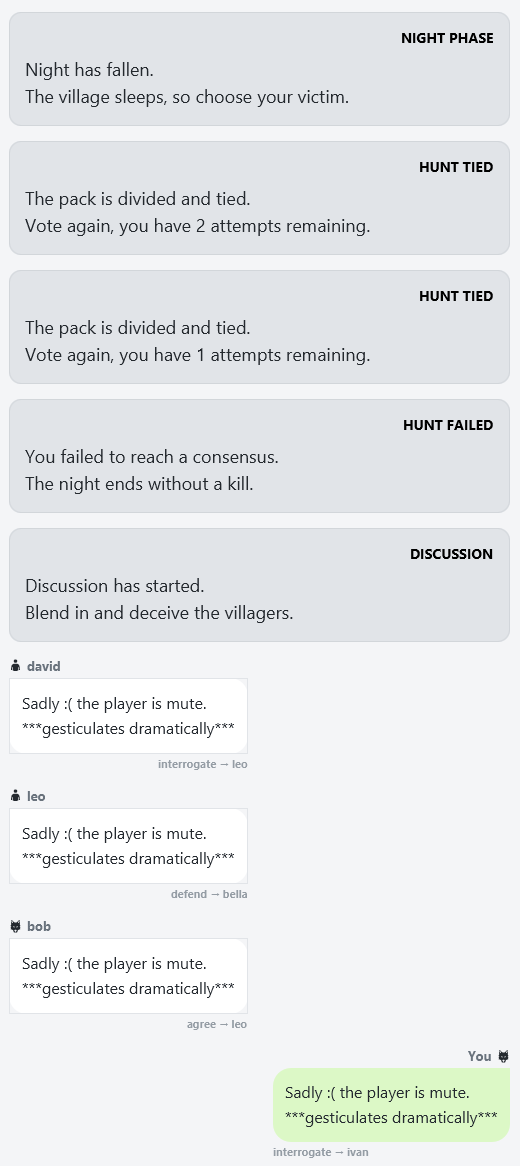
\includegraphics[width=\textwidth]{images/chat_no_llm.PNG} % Update with your actual filename
        \caption{Without LLM: Rigid, prefab messages lacking immersion.}
        \label{fig:chat_no_llm}
    \end{subfigure}
    \hfill
    % Right side: With LLM
    \begin{subfigure}[b]{0.48\textwidth}
        \centering
        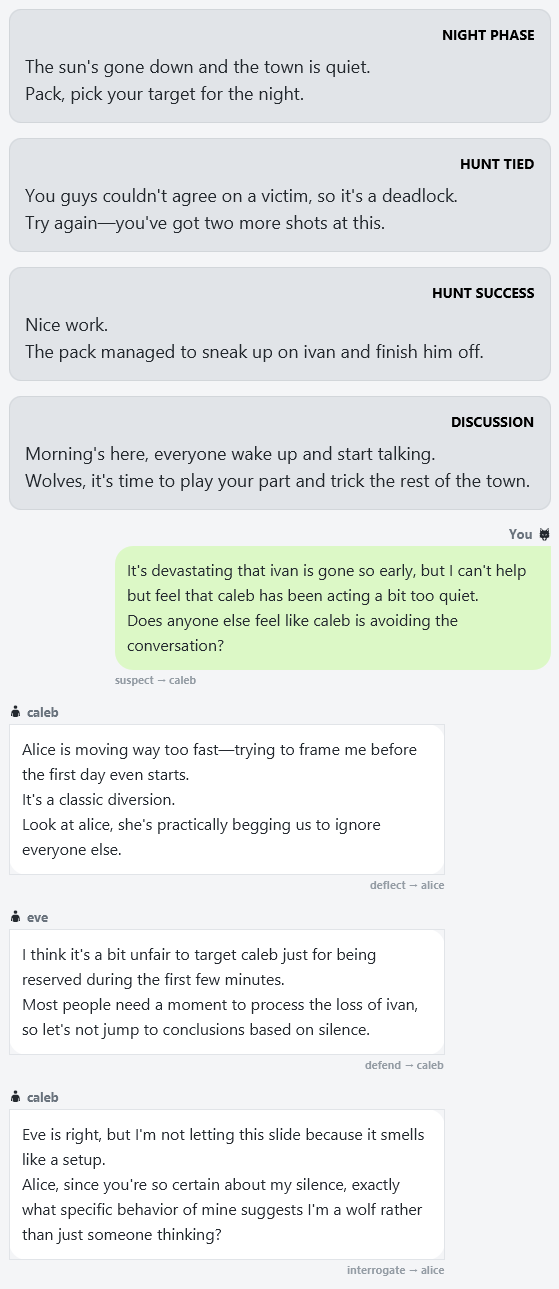
\includegraphics[width=\textwidth]{images/chat_llm.PNG} % Update with your actual filename
        \caption{With LLM: Organic, immersive dialogue for both players and the Narrator.}
        \label{fig:chat_with_llm}
    \end{subfigure}
    
    \caption{Comparison of the game's chat interface. The integration of the LLM transforms the interaction from abstract speech acts (left) into a narrative roleplay experience (right).}
    \label{fig:llm_chat_comparison}
\end{figure}

To bridge the gap between abstract symbolic reasoning and human-readable roleplay, the architecture integrates a \textbf{Large Language Model} to generate  immersive dialogue. To avoid API costs, the proposed bridge connects strictly to local models, hosted using \textbf{Ollama}, interfaced through a custom Java wrapper (\texttt{src/llm/OllamaAPI}).

\paragraph{Verifying Connectivity and Model Warm-up}
Before any text generation occurs, the system must validate the local LLM environment. During the Narrator's boot sequence, the agent executes a custom internal action (\texttt{llm.ping\_llm}) to establish a handshake with the Ollama server. This ping serves three critical architectural purposes:

\begin{enumerate}
    \item \textbf{GPU Warm-up:} By default, Ollama loads models into memory only when queried, which introduces severe "cold-start" latency on the first request. The ping explicitly passes the \texttt{"keep\_alive":-1} parameter in its JSON payload, forcing the Ollama server to load the requested model directly into VRAM and hold it there indefinitely, to ensure faster response time.
    
    \item \textbf{Model Validation:} It verifies that the Ollama service is actively running on the local port and that the specific model requested by the simulation settings is actually installed on the machine.
    
    \item \textbf{Error Handling:} If the connection is refused or the model is missing, the Java API catches the exception and returns a specific error string to the Jason environment. This allows the multi-agent system to safely abort the LLM initialization and disable any module that requires it. By catching this during the warm-up phase, the simulation can seamlessly fall back to the "bland" symbolic logging mode without crashing mid-game.
    
\end{enumerate}


\subsection{Prompting the LLM}
\label{subsec:llm_communication}

The communication layer that bridges the Jason logic and the LLM is handled by two dedicated Java classes: \texttt{LLMUtils} and \texttt{OllamaAPI}. In this architecture, the logical content of the prompt is determined entirely within Jason, while the Java layer simply glues together and sanitizes the strings. The assembled prompt is then sent to the LLM, and finally, the result is post-processed to ensure a safe output.

\begin{figure}[H]
    \centering
    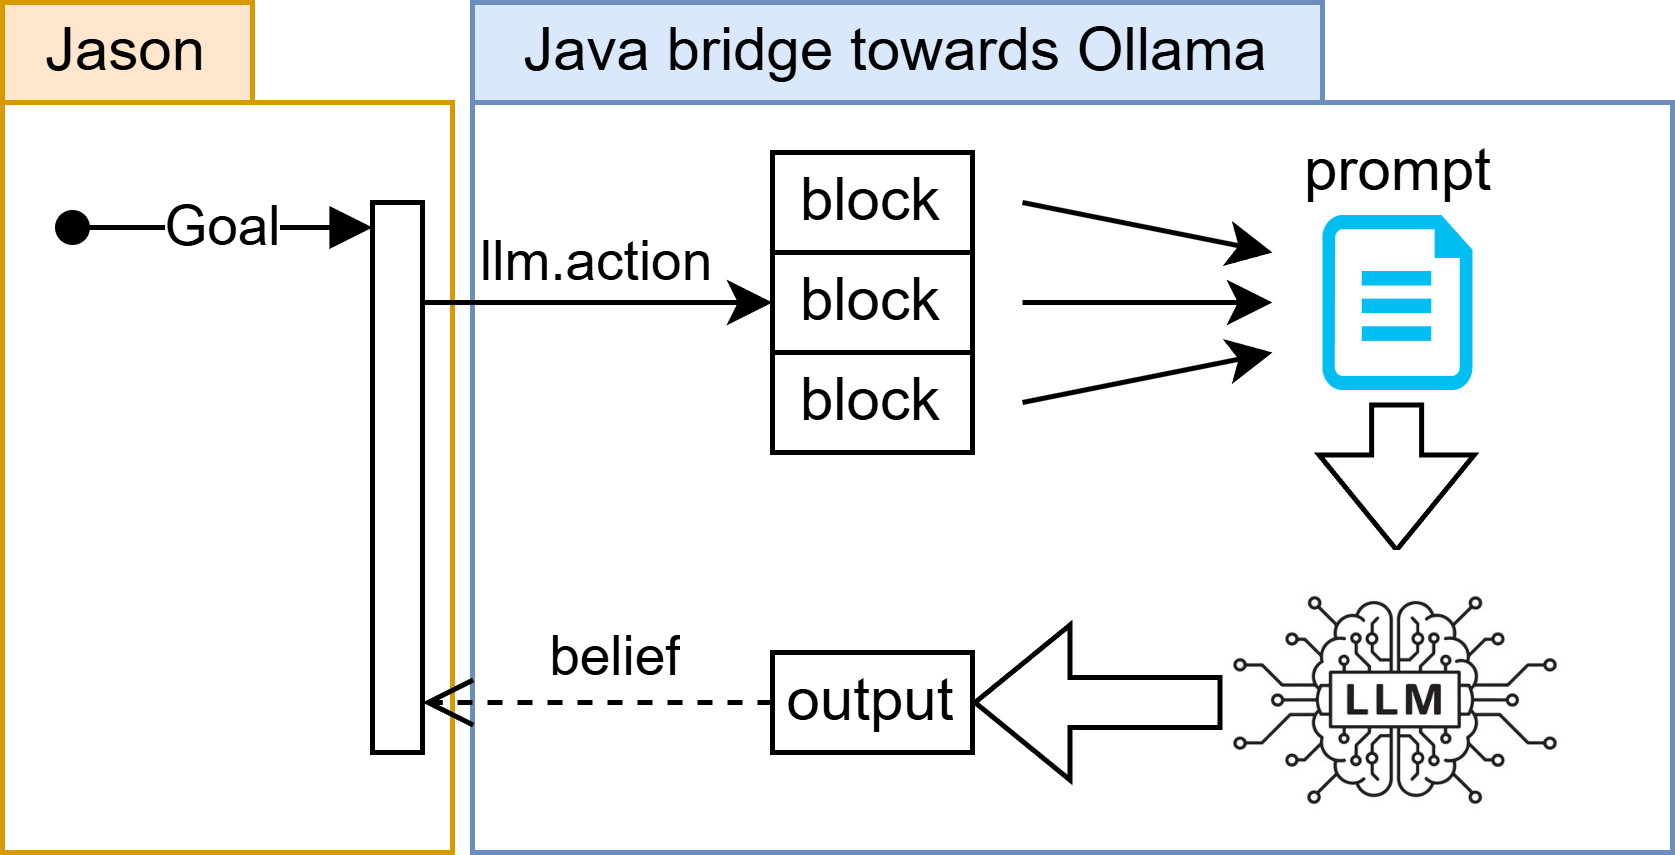
\includegraphics[width=0.8\textwidth]{images/ollama_bridge.png}
    \caption{Interaction between the Jason Engine and the Ollama API. A custom Java action is called by passing ``building blocks'' as input; they are merged into a prompt given to the LLM, and the output is directly injected as a belief into the agent.}
    \label{fig:ollama_bridge}
\end{figure}

To streamline query management, the system utilizes \texttt{LLMUtils.PromptBuilder}, which constructs prompts by appending modular text blocks to improve code reusability.

Once the full prompt is assembled, it is routed to the \texttt{OllamaAPI}. This class wraps the prompt into a JSON payload and issues an HTTP POST request directly to the local model. Once the response is received, the class extracts the generated text and, if configured, saves the full interaction payload to a local directory for later debugging and analysis. The raw output is then routed back through \texttt{LLMUtils}, which sanitizes the text to prevent parsing failures. The sanitized string is wrapped into a Jason \texttt{Literal} and asynchronously injected into the agent's belief base, triggering a \texttt{wakeUpSense()} call to immediately resume the agent's execution cycle.

\paragraph{Stateless Execution Bottleneck}
A critical observation is that the LLM is treated as a purely stateless function. The \texttt{OllamaAPI} does not maintain hidden states or conversation memory between calls\footnote{This implementative choice is defined by the way the LLM reasoner was designed: each action is completely independent, and the only state kept between them must be explicitly defined as a Jason belief. Furthermore, the Ollama API must be completely agnostic to the game size; hence, keeping a conversation open for each player could result in a VRAM shortage.}. Consequently, every request is atomically independent, requiring the prompt to redefine the complete context from scratch. While the model remains pre-loaded in the GPU, handling concurrent queries with massive contextual payloads renders the system highly susceptible to computational bottlenecks (as highlighted in Section \ref{sec:results}).


\paragraph{Bridging Symbolic Logic and Natural Language}
A substantial portion of the development effort was dedicated to the non-trivial challenge of designing an explicit, deterministic encoding that translates the agents' hidden symbolic states (i.e the Agent's beliefs) into flexible natural language prompts. To ensure contextual accuracy and narrative immersion, the language model required absolute integrity regarding the current game state. 

However, strict hardware limitations constrained the architecture to rely on smaller LLMs: these compact models proved highly susceptible to \textbf{contextual drift and catastrophic hallucination} when exposed to specific token or overloaded context windows\footnote{A example of this contextual drift that can be appreciated on the tested model is provided in Section \ref{sec:results}.}. Consequently, crafting modular prompts  rigid enough to prevent hallucination, yet flexible enough to cover  each possible state of the game, required extensive (both temporal and testing-wise) iterative trial-and-error. The Prompt defined in the next parts are hence the results of this long process.

\subsection{Enhancing Narration}
\label{subsec:llm-narration}
As detailed in Section \ref{sec:narrator}, the transition along the edges of the game's state machine is strictly managed by the Narrator. In the baseline implementation, state transitions are broadcastes using hard-coded messages, stored in \\
\texttt{narrator/core/game\_narration.asl}. These default templates are parametric and defined by a unique identifier, a phase title, a specific conversational intent (the core speech act it must convey), and a default base message.

\begin{lstlisting}[frame=single, language=Prolog, caption={Example of a parametric narration template. The rule dynamically binds variables to generate the title, intent, and default message.}, label={lst:narrator_msg_template}]
narrator_message(exec_result,[villagers, villager, Victim], PhaseTitle, PhaseIntent, Message) :-
    PhaseTitle = "Execution Result - Failure" &
    .concat("Announce to the village that the executed player ", Victim, " was an innocent villager.", PhaseIntent) &
    .concat("A tragic mistake. The town executed ", Victim, ", an innocent villager.", Message).
\end{lstlisting}

If the LLM module is enabled, the agent dynamically aggregates its predefined speaking style, retrieves the most recent phase logs, and translates them into a human-readable context block. 

\begin{lstlisting}[frame=single, language=Prolog, caption={Simplified dispatch logic for the Narrator. It retrieves the required context and asynchronously queries the Java API, safely falling back to the base message if the LLM generation fails.}, label={lst:narrator_dispatch}]
?msg(_, BaseMessage, PhaseTitle, PhaseIntent, _);
if (setting(llm_narrator(true))) {
    ?narrator_style(StyleDesc);
    ?setting(narrator_chunk_log_size(NarratorChunkLogSize));
    ?get_log_chunk(any, TargetList, NarratorChunkLogSize, LogChunk);
    ?translate_log(LogChunk, LogChunkTranslated);
    
    llm.narrator_message(PhaseIntent, BaseMessage, StyleDesc, LogChunkTranslated);
    .wait(narrator_result(FinalMessageString));
    -narrator_result(_);
} else {
    FinalMessageString = BaseMessage;
};
\end{lstlisting}

The \texttt{StyleDesc} variable is populated by a hard-coded belief that dictates the Narrator's persona, ensuring a consistent ``tabletop game master'' tone throughout the Game.

\begin{lstlisting}[frame=single, language=Prolog, caption={The Narrator's style definition explicitly outlines the tone, vocabulary, and prohibitions.}, label={lst:narrator_style}]
narrator_style(Desc) :- 
    .concat("- TONE: Conversational, engaging, slightly dramatic but clear.\n",
            "- VOCABULARY: Natural tabletop language (e.g., 'You guys', 'The village'). Use contractions.\n",
            "- FOCUS: Setting the mood while delivering phase mechanics.\n",
            "- PROHIBITION: DO NOT sound like a robotic terminal. DO NOT use overly formal words.", 
            Desc).
\end{lstlisting}

Finally, the extracted data blocks ( the intent, the base message, the style description, and the translated history log) are passed to the custom Java internal action \texttt{llm.narrator\_message}. This wrapper utilizes the \texttt{PromptBuilder} utility to construct the structured prompt, appending each piece of data into modular text blocks.

\newpage
\begin{lstlisting}[frame=single, basicstyle=\scriptsize\ttfamily, breaklines=true, caption={The fully assembled prompt sent to the Ollama API. Each block is vital to prevent the LLM from hallucinating or copying the messages sent before.}, label={lst:narrator_prompt}]
### WORLD SETTING
You are participating in a multi-agent simulation of the game Werewolf/Mafia.

### YOUR IDENTITY
ROLE: TABLETOP GAME MASTER / NARRATOR

### STYLE OF SPEECH
- TONE: Conversational, engaging, slightly dramatic but clear.
- VOCABULARY: Natural tabletop language. Use contractions.
- FOCUS: Setting the mood while delivering phase mechanics.
- PROHIBITION: DO NOT sound like a robotic terminal. DO NOT use overly formal words.

### REFERENCE MESSAGE
A tragic mistake. The town executed heidi, an innocent villager

### YOUR CURRENT GOAL
INTENT TO CONVEY: Announce to the village that the executed player heidi was an innocent villager.

### RECENT DIALOGUE HISTORY 
- [NARRATOR]: Tough break, guys. You just kicked out Frank, and he was totally innocent.
- [NARRATOR]: Lights out, everybody. Try to stay safe while the pack begins their hunt.
- [NARRATOR]: Rise and shine, folks. It's a grim start to the day because Ivan was taken out...
- [NARRATOR]: Alright, floor's open. Start digging into each other and root out the monsters!
- [NARRATOR]: Discussion's closed. It's time to lock in your choices!

### RESPONSE CONSTRAINTS (MANDATORY)
1. STRICT LIMIT: Output 1 to 3 sentences maximum.
2. NO PARROTING: Use the REFERENCE MESSAGE strictly for factual pacing. Write entirely new dialogue.
3. VOCABULARY VARIATION: You are strictly forbidden from using opening greetings present in the HISTORY.
4. NO REPETITION: Do not reuse any specific wording from the HISTORY nor the REFERENCE MESSAGE.
5. ASSUMED CONTEXT: Focus strictly on the INTENT TO CONVEY. Assume players possess full knowledge of past events.
6. FORMAT: Output ONLY the raw response string. No meta-commentary, no JSON, no markdown.
7. ONE-LINE: The output must be a single line of text, without line breaks or paragraphs.

GENERATE RESPONSE NOW:
\end{lstlisting}


\paragraph{Empirical Prompt Tuning}
During development, empirical testing revealed that each discrete block within the prompt structure is critical for stabilizing the output of the quantized LLM. Specifically:
\begin{itemize}
    \item \textbf{\texttt{\#\#\# STYLE OF SPEECH}:} Mitigates the model's inherent verbosity and enforces strict role-playing boundaries, preventing out-of-character responses.
    \item \textbf{\texttt{\#\#\# REFERENCE MESSAGE}:} Acts as a \textbf{One-Shot} learning anchor. Testing demonstrated that relying solely on the \texttt{INTENT} causes massive hallucination; giving a structural baseline grounds the text generation.
    \item \textbf{\texttt{\#\#\# RECENT DIALOGUE HISTORY}:} Serves as a negative constraint to prevent repetitive phrasing. However, testing also revealed a strict trade-off: passing an excessively large log chunk overwhelms the small model's attention span, causing it to parrot previous lines rather than generate novel text.
    \item \textbf{\texttt{\#\#\# RESPONSE CONSTRAINTS}:} Enforces rigid syntactic formatting, ensuring the raw output string integrates organically into the Java UI chat panel without breaking the display logic.
\end{itemize}

\subsection{LLM Reasoner (Ollama)}
\label{subsec:llm-reasoner}
Building on the logic used for the Narrator's message enhancement, it is possible to define the final type of reasoner: the LLM-powered reasoner. To minimize modifications to the Symbolic Reasoner's architecture, is kept the same blueprint for its internal state, defined by the agent's self-awareness beliefs and Trait Matrix (and also other internal beliefs). However, in this context, we require a \textbf{textual encoding} process to convert these symbolic values into \textbf{blocks} that can be used to construct the prompt.

\subsubsection{Textual Encoding of the Agent State}
\label{subsubsec:llm-reasoner-encoding}
The files responsible for this symbolic-to-text translation are modularly organized within the \texttt{shared/llm\_context/} directory. Rather than relying on a single monolithic parser, each script is dedicated to decoding a specific dimension of the agent's knowledge base, such as conversation history, active traits, or psychological temperament. Each files operates indipendenlty and is loaded at  runtime (if needed), during the player's initialization.

\paragraph{\textbf{\texttt{log\_2\_context.asl}}} 
This module handles the integral log stored by the narrator in its belief base. It defines the core rule \texttt{translate\_log(LogChunk, TextualEncoding)}, that given a raw list of the Narrator's log events, encodes it in a list of text lines. Because the log is structured as a sequence of nested Prolog literals (e.g., \texttt{action(speech(...))}), the rule recursively iterates through the list, pattern-matching specific game events and mapping them to predefined string templates. Finally, it concatenates these translated entries into a single, chronologically formatted text block. 

\begin{verbatim}
log_to_text(action(speech(Src, Msg, Int)), S) :-
    .concat("- [", Src, " -> ", IntStr, "]: ", Msg, S).

log_to_text(action(victim(hunt, Vic, R)), S) :-
    .concat("    - ", Vic, ", a ", R, 
            " was killed by the hunt of the wolves.", S).

log_to_text(action(victim(vote, Vic, R)), S) :-
    .concat("    - ", Vic, ", a ", R, 
            " was eliminated by the village.", S). 

log_to_text(action(hunt_vote(Src, Tgt)), S) :-
    .concat("    - ", Src, " hunted ", Tgt, S).

log_to_text(action(vote(Src, Tgt)), S) :-
    .concat("    - ", Src, " voted for ", Tgt, S).
\end{verbatim}

\paragraph{\textbf{\texttt{performatives\_2\_context.asl}}} 
It defines a set of rules to translate the (abstract) speech acts into explicit natural language instructions. It maps each symbolic performative to a precise behavioral instruction detailing how the LLM should construct its message. The rules are parametric in the Player's Name, to define a explicit guide for the LLM. The defined mappings are as follows:

\begin{itemize}
    \item \textbf{\texttt{accuse(\{PLAYER\})}:} 
        ``Aggressively accuse \{PLAYER\} of being a wolf and push the village to execute them.''
    \item \textbf{\texttt{defend(\{PLAYER\})}:} 
        ``Defend \{PLAYER\} against current suspicions and argue for their innocence.''
    \item \textbf{\texttt{suspect(\{PLAYER\})}:} 
        ``Express heavy suspicion towards \{PLAYER\} without fully committing to an accusation.''
    \item \textbf{\texttt{agree(\{PLAYER\})}:} 
        ``Strongly agree with the recent statements or tactical direction of \{PLAYER\}.''
    \item \textbf{\texttt{interrogate(\{PLAYER\})}:} 
        ``Ask a direct, pressuring question to \{PLAYER\} to force them into a mistake or contradiction.'
    \item \textbf{\texttt{deflect(\{PLAYER\})}:} 
        ``Deflect any current suspicion away and firmly redirect the village's attention onto \{PLAYER\}.''
\end{itemize}


\paragraph{\textbf{\texttt{traits\_2\_context.asl}}} 
This module translates the agent's epistemic belief matrix into a structured psychological context block. It first formally describes the active traits in natural language, dynamically adapting the definitions based on the agent's assigned role:

\begin{itemize}
    \item \textbf{\texttt{suspicion}} (Villagers only): ``A low level means you believe they are innocent and trustworthy, while a bigger value means you strongly suspect they are a wolf.''
    \item \textbf{\texttt{threat}} (Wolves only): ``A low level means they are ignoring you or pose no danger, while a bigger value means they are actively attacking you or your pack.''
    \item \textbf{\texttt{utility}}: ``A low level means they are an obstacle or useless to your strategy, while a bigger value means they are actively helpful to your goals.''
    \item \textbf{\texttt{influence}}: ``A low level means they are losing credibility or looking foolish, while a bigger value means they are highly persuasive and leading the game.''
\end{itemize}

Second, it aggregates the current numerical trait values for every other player into a formatted list. A critical implementation detail is the explicit randomization of the player array (using \texttt{.shuffle}) prior to converting the players' profiles into text. This step is necessary to mitigate the LLM's inherent \textbf{positional bias} toward specific players\footnote{This highlights a key observation discussed in Section \ref{sec:results}: this mitigation strategy alone is insufficient to shift the LLM's inherently biased decision-making process toward a completely agnostic (equiprobable) distribution.}.

Furthermore, since the traits are lazily evaluated, some players might not have any defined traits at a given moment. To account for this missing data, an explicit string is appended on top of the prompt instructing the LLM on how to interpret the absence of values.


\begin{lstlisting}[frame=single, basicstyle=\footnotesize\ttfamily, breaklines=true, caption={Example of the generated trait context block for a wolf agent. Not each trait of the players is defined, and only the ``alive'' ones are listed.}, label={lst:traits_context}]
    CURRENT EPISTEMIC OPINIONS TOWARDS OTHER PLAYERS:
    NOTE: Any traits not listed is 0.0 (Unbiased/Neutral opinion)
    
    ivan(influence: 0.41, utility: 0.38, suspicion: 0.11)
    judy(utility: 0.11, influence: 0.05)
    arthur(influence: 0.41)
    bob(suspicion: 0.53, influence: 0.13)
    grace(suspicion: -0.15, utility: 0.12, influence: 0.03)
    kevin(utility: 0.51)
    eve(suspicion: 1, influence: 0.53)
\end{lstlisting}


\paragraph{\textbf{\texttt{temper\_2\_context.asl}}} 
Is the module accountable for the translation of the agent's self-aware metrics. It is divided into two distinct parts. The first part defines the player's constant personality traits, including their role, name, and static moods. To convert continuous numerical values into human-readable text, each mood's domain is discretized into five bins. Each bin maps directly to an explicit behavioral archetype.

\begin{lstlisting}[frame=single, basicstyle=\footnotesize\ttfamily, breaklines=true, caption={Discretization of the continuous \texttt{paranoia} trait into five distinct behavioral bins. The \texttt{ProAgent} engine evaluates the numerical value to select the appropriate natural language description.}, label={lst:paranoia_bins}]
@paranoia_very_high[ temper([paranoia(1.0)]) ]
+!compile_paranoia_rule(Rule) 
    <-  .concat("- CONSPIRACIST: You are a true conspiracist. You trust absolutely no one (except your own packmates, if any), assume every statement is a trap, and see conspiracies everywhere.", Rule).

@paranoia_high[ temper([paranoia(0.5)]) ]
+!compile_paranoia_rule(Rule) 
    <-  .concat("- SKEPTIC: You are a sharp skeptic. You scrutinize others' words closely looking for hidden motives and rarely take things at face value.", Rule).

@paranoia_neutral[ temper([paranoia(0.0)]) ]
+!compile_paranoia_rule(Rule) 
    <-  .concat("- REALIST: You are a grounded realist. You are cautious but willing to listen to reason and evaluate evidence fairly.", Rule).

@paranoia_low[ temper([paranoia(-0.5)]) ]
+!compile_paranoia_rule(Rule) 
    <-  .concat("- OPTIMIST: You are a hopeful optimist. You are trusting, hence you generally take people at their word and assume good intentions.", Rule).

@paranoia_very_low[ temper([paranoia(-1.0)]) ]
+!compile_paranoia_rule(Rule) 
    <-  .concat("- NAIVE: You are completely naive. You are highly trusting, implicitly believe what others tell you, and tend to ignore red flags.", Rule).
\end{lstlisting}

During player initialization, the \texttt{vesna.ProAgent} parsing logic evaluates these static temperaments, extracts the corresponding text definitions, and permanently store them within a \texttt{+player\_description(ProfileBlock)} belief to avoid redundant string concatenation during gameplay.


\begin{figure}[H]
    \centering
    
    % Top: Topology Scatter Plot
    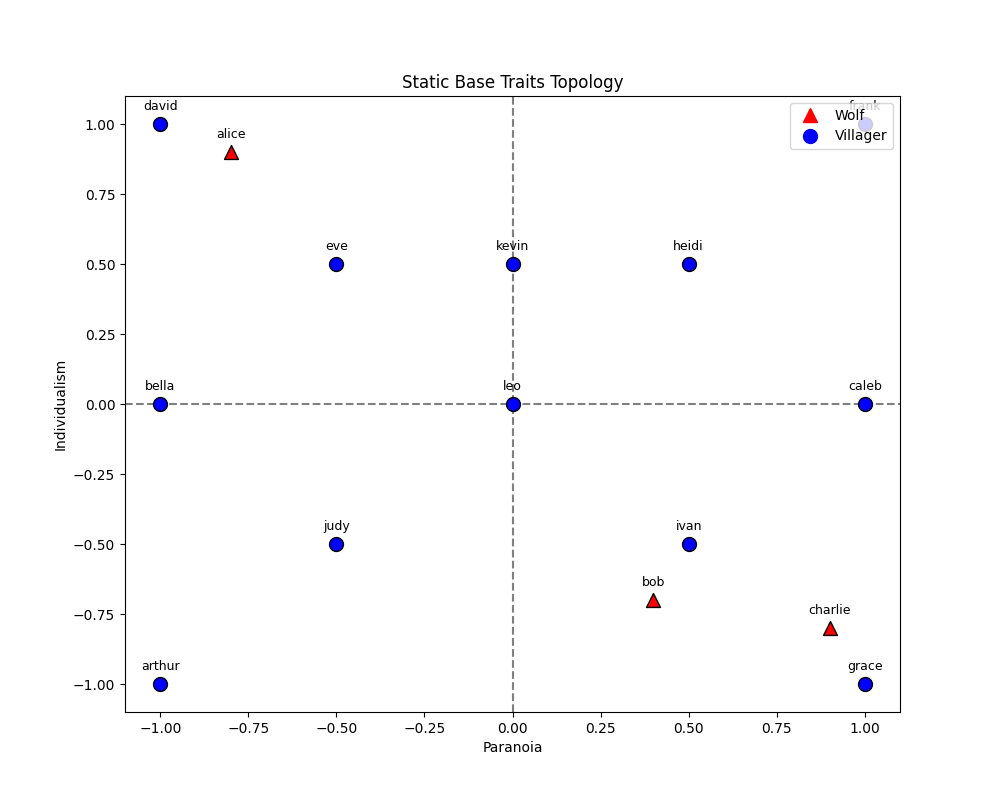
\includegraphics[width=1\textwidth]{images/personality topology.png}
    
    \vspace{1.5em} % Structural spacing between image and text blocks
    
    % Bottom: Two-column tabular for guaranteed full-height vertical divider
    \begin{tabular}{@{} p{0.47\textwidth} | p{0.47\textwidth} @{}}
        \scriptsize
        \textbf{Player Name:} alice \newline
        \textbf{Hidden Role:} wolf \newline
        \textbf{Personality Profile:}
        \begin{itemize}
            \item \textbf{NAIVE:} You are completely naive. You are highly trusting, implicitly believe what others tell you, and tend to ignore red flags.
            \item \textbf{MAVERICK:} You are a true maverick. You completely ignore the consensus of your peers, vote and act based solely on your own deductions, and refuse to follow the group.
        \end{itemize}
        &
        \scriptsize
        \textbf{Player Name:} grace \newline
        \textbf{Hidden Role:} villager \newline
        \textbf{Personality Profile:}
        \begin{itemize}
            \item \textbf{CONSPIRACIST:} You are a true conspiracist. You trust absolutely no one (except your own packmates, if any), assume every statement is a trap, and see conspiracies everywhere.
            \item \textbf{CONFORMIST:} You have a strict pack mentality. You blindly follow the choices and votes of your peers to maintain absolute unity, completely disregarding your own beliefs.
        \end{itemize}
    \end{tabular}
    
    \caption{Translation of static traits into explicit LLM prompt blocks. The exact initial spatial coordinates for agents like Alice (\texttt{paranoia}: $-0.8$, \texttt{individualism}: $0.9$) and Grace (\texttt{paranoia}: $1.0$, \texttt{individualism}: $-1.0$) define the selection of the behavioral archetypes.}
    \label{fig:traits_to_profile}
\end{figure}


\paragraph{\textbf{Speech modeling based on dynamic moods}} 
The second objective of the \texttt{temper\_2\_context.asl} module is to guarantee rhetorical guidelines during \textbf{Natural Language Generation}. The agent's speech style is structured using a hybrid prompt block: a static component that establishes broad tonal directions and explicit prohibitions (designed to inhibit the LLM's inherent stylistic biases), and a dynamic component driven by the agent's active mood variables. 

The selection logic is a the same as the previously described pipeline, utilizing the engine to extract the appropriate rhetorical goals based on real-time moods. Specifically, each injected mood string provides both a soft description of the agent's psychological state and rigid syntactic constraints that the LLM must follow to ensure immersive roleplay.

\begin{lstlisting}[frame=single, basicstyle=\footnotesize\ttfamily, breaklines=true, caption={Example of a generated speech style block. The dynamic parameters for STRESS LEVEL and SOCIAL EXPOSURE are evaluated and injected at execution time based on the agent's internal state.}, label={lst:style_of_speech}]
### STYLE OF SPEECH
- TONE: Analytical, natural. Speak like an intelligent adult in a high-stakes board game.
- STRESS LEVEL (CRITICAL): You are in a state of high panic.
  SYNTAX GUIDELINES: Speak in rushed, fragmented bursts. Use short sentences and occasional dashes (-) to show racing thoughts, but DO NOT sound cartoonish or repeat the same phrases (like 'I didn't'). Keep the vocabulary natural but urgent.
- SOCIAL EXPOSURE (NEUTRAL):You are blending into the background.
  RHETORIC GUIDELINES: Participate by asking probing questions or evaluating evidence collectively. Avoid making hard, bold declarations that would draw unnecessary attention to you.
- PROHIBITION: NO robotic academic declarations (like furthermore, therefore).
- PROHIBITION: NO cartoonish stuttering, exaggerated catchphrases, or repetitive dialogue loops. Adapt dynamically to the context.
\end{lstlisting}

Conversely, during different cognitive cycles—such as when the LLM is prompted to evaluate and update the agent's self-aware opinions regarding its own state—these continuous metrics must be formally explained rather than applied as immediate behavioral constraints. This is achieved through explicit natural language formalizations mapping the numerical domain to semantic meaning.

\begin{itemize}
    \item \textbf{\texttt{stress}:} ``A low level means you feel relieved, secure, or in control, while a bigger value means you feel panicked, pressured, or fear elimination.''
    \item \textbf{\texttt{exposure}:} ``A low level means you feel hidden, ignored, or successfully blend in, while a bigger value means you are thrust into the spotlight and suspected.''
\end{itemize}


\subsubsection{Updating the World Model}
Now that we have introduced the building blocks, we can describe how the Reasoner responds to external events. Figure \ref{fig:llm_reasoner_read} illustrates the  pipeline: symbolic beliefs are converted into textual building blocks, merged into a prompt, processed by the LLM, and then translated back into symbolic updates.

\begin{figure}[H]
    \centering
    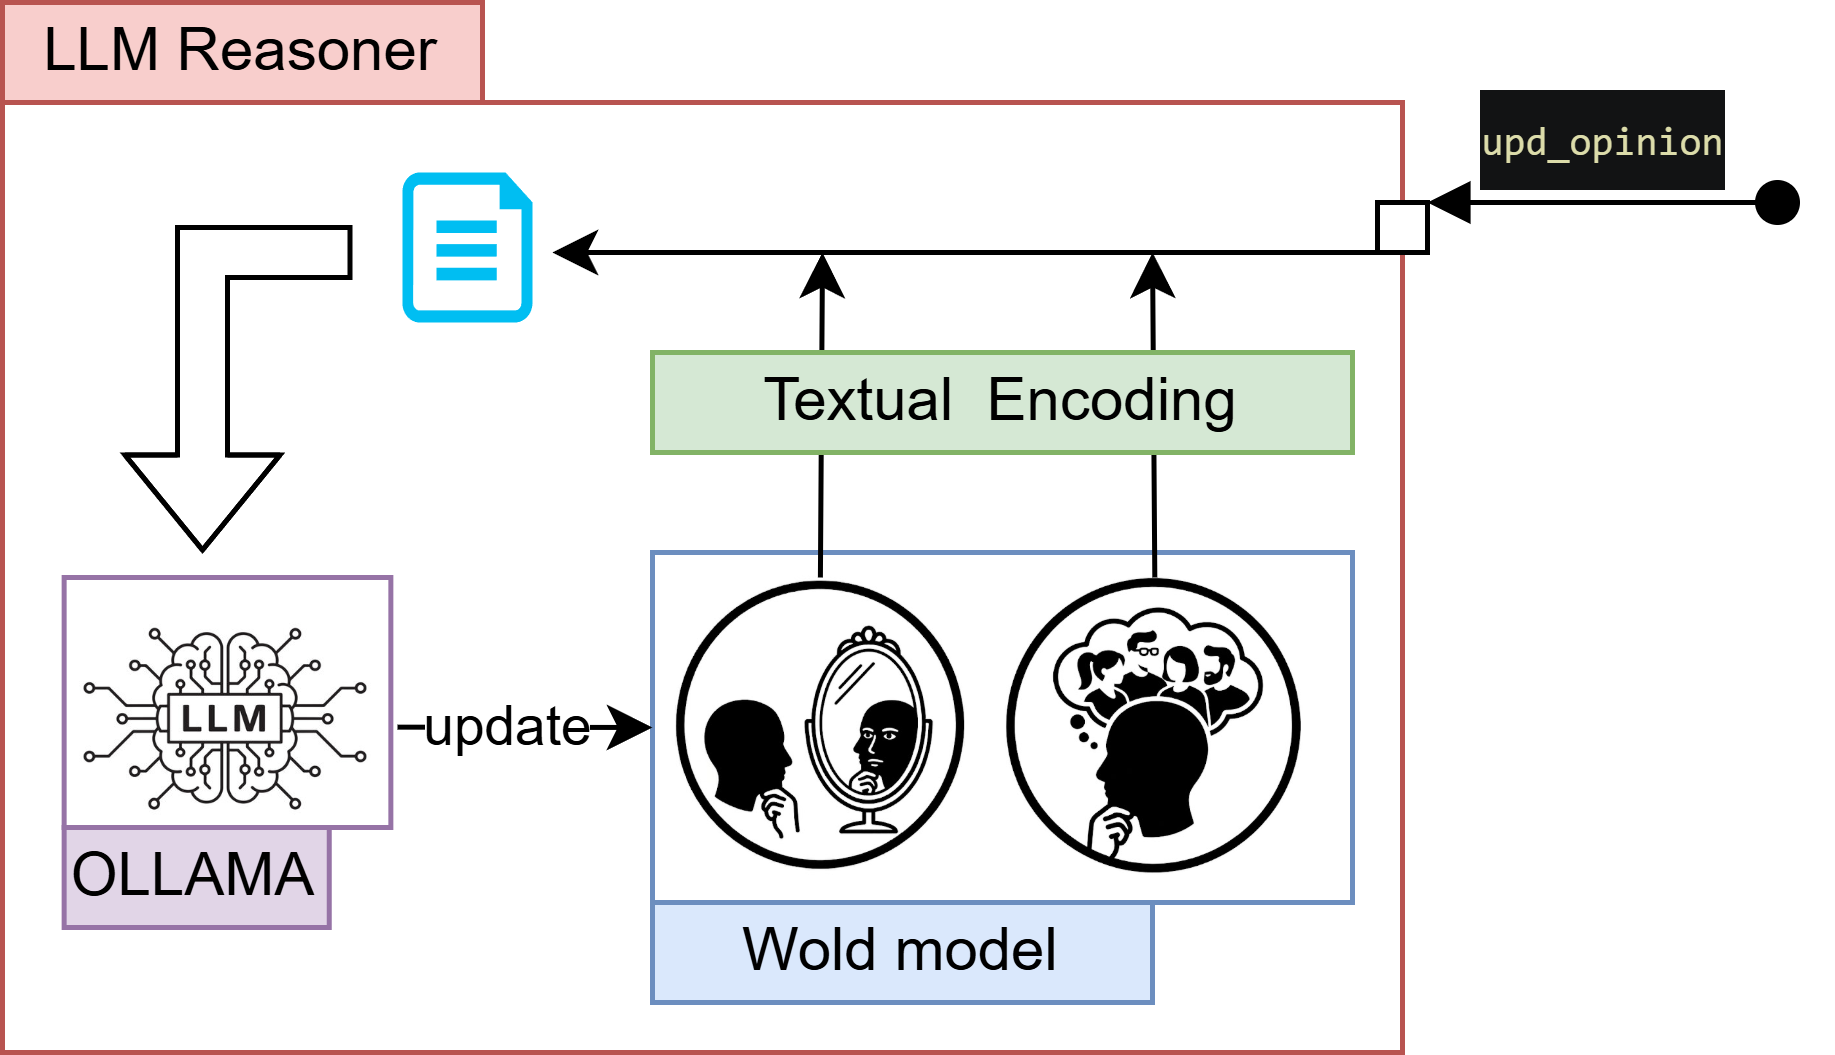
\includegraphics[width=0.8\textwidth]{images/llm_reasoner_write_on.png}
    \caption{Passive Belief's update by the Reasoner. A custom Java action is called by passing textual ``building blocks'' as input; they are merged into a prompt given to the LLM, with the output used to update the internal World Model of the Agent.}
    \label{fig:llm_reasoner_write_on}
\end{figure}

The orchestration logic in \texttt{reasoner/llm/update\_opinions.asl} counters the LLM's inherent stochasticity with robust retry mechanisms. Queries retry up to $K$ times upon failure\footnote{A common issue given the strict requirement for a perfectly formatted Jason list.}, while fallback goals (\texttt{-!invoke\_llm\_opinions}) catch exceptions to prevent system deadlocks. 

Furthermore, to avoid asynchronous race conditions when agents process multiple events concurrently, the plan dynamically generates a unique identifier (\texttt{UID}) for each LLM call (Listing \ref{lst:llm_concurrency}).

\begin{lstlisting}[frame=single, language=Prolog, caption={Implementation of concurrent execution safety. A unique identifier is generated to map the asynchronous LLM response back to the specific execution thread.}, label={lst:llm_concurrency}]
.random(RandNum);
.concat("UID_", RandNum, UID);

//call the async action, giving the blocks
llm.update_opinions(UID, IdentityContext, TraitsOpinionsString, LLMFriendlyLog, WolfPackStr, ActionStr, TraitsListStr, MoodsListStr);
        
//await the specific beliefdefined by UID
.wait(opinions_result(UID, UpdatesString));

//remove, since no more useful
-opinions_result(UID, _);
\end{lstlisting}

This ensures that the \texttt{.wait()} operator only resumes when the custom Java action injects the target belief signature matching the specific thread's \texttt{UID}, preventing the multi-agent system from deadlocking or mixing up responses.

\vspace{1em}

\begin{lstlisting}[frame=single, basicstyle=\scriptsize\ttfamily, breaklines=true, caption={Example of a complete prompt used to obtain a set of updates to apply to the agent's moods and epistemic traits.}, label={lst:upd_opinion_prompt}]
### WORLD SETTING
You are participating in a multi-agent simulation of the game Werewolf/Mafia.

### YOUR IDENTITY
Player Name: bob
Hidden Role: wolf
Personality Profile:
- SKEPTIC: You are a sharp skeptic. You scrutinize others' words closely looking for hidden motives and rarely take things at face value.
- COLLABORATIVE: You are a team player. You prefer to align your votes and targets with your peers, often setting aside your personal suspicions to ensure a unified front.

### YOUR CURRENT INTERNAL STATE (MOOD)
- stress: Current value is 0.5. A low level means you feel relieved, secure, or in control, while a bigger value means you feel panicked, pressured, or fear elimination.
- exposure: Current value is 0.5. A low level means you feel hidden, ignored, or successfully blend in, while a bigger value means you are thrust into the spotlight and suspected.

### YOUR CURRENT OPINIONS OF OTHERS (TRAITS)
HOW TO READ THESE VALUES:
- threat: A low level means they are ignoring you or pose no danger, while a bigger value means they are actively attacking you or your pack.
- utility: A low level means they are an obstacle or useless to your strategy, while a bigger value means they are actively helpful to your goals.
- influence: A low level means they are losing credibility or looking foolish, while a bigger value means they are highly persuasive and leading the game.

CURRENT EPISTEMIC OPINIONS TOWARDS OTHER PLAYERS:
NOTE: Any traits not listed in a player's profile is currently 0.0 (Unbiased/Neutral opinion).
eve(threat: 1, utility: -0.5, influence: 0.18)
kevin(threat: 0.69, utility: 0.72)
grace(influence: 0.23, utility: 0.22, threat: 0.32)
ivan(utility: 0.36, threat: 0.16)
leo(threat: 0.5, influence: 0.07)
arthur(threat: 0.56, utility: 0, influence: -0.04)
judy(threat: 0.48, utility: -0.43)

### SECRET KNOWLEDGE ABOUT THE PACK
Your Wolf Pack: bob.
You MUST pretend to be a normal villager in public.
NEVER reveal your pack.

### LATEST EVENTS
- [NARRATOR]: The stars are out and the town's gone quiet. Wolves, decide who's not waking up tomorrow.

### MOST RECENT ACTION (TO BE EVALUATED)
arthur casts a vote to eliminate eve

### YOUR CURRENT GOAL
TASK: Evaluate the psychological and strategic impact of the MOST RECENT ACTION on your internal opinions and mood.
EFFECT: The output will directly update your traits (opinions of others) and mood (internal state) which will influence your future decisions and interactions in the game.
MOTIVATION: This is a critical step for adapting your strategy as the game evolves, since it directly affects your ability to navigate the social dynamics of the game.

### RESPONSE CONSTRAINTS (MANDATORY)
1. OUTPUT FORMAT: You MUST output exactly a Jason list of literals. Do NOT output markdown, backticks, or any explanation. No preambles.
2. LITERAL FORMATS:
   - To update a player's trait: trait_update(player_name, attribute, delta)
   - To update your own mood: mood_update(attribute, delta)
3. VALID ATTRIBUTES: Use ONLY the traits and moods explicitly defined in the blocks above (YOUR CURRENT INTERNAL STATE (MOOD) and YOUR CURRENT OPINIONS OF OTHERS (TRAITS)).
4. SCALE BOUNDARIES (CRITICAL): All traits and moods exist on a hard scale from -1.0 to 1.0.
5. DELTA VALUES: Use float values between -0.5 and 0.5 to shift the current values. You MUST use NEGATIVE values for relief, lost influence, or reduced threat, and POSITIVE values for increases.
6. ZERO-IMPACT FALLBACK: If the action has no logical impact, output: []
7. SYNTAX EXAMPLE: [trait_update(AGENT_NAME, ATTRIBUTE, FLOAT), mood_update(ATTRIBUTE, FLOAT)]

GENERATE RESPONSE NOW:
\end{lstlisting}

As detailed in the previous sections, it dynamically maps the agent's symbolic beliefs into precise textual blocks. The fixed guidelines at the end of the prompt (\texttt{\#\#\# YOUR CURRENT GOAL} and \texttt{\#\#\# RESPONSE CONSTRAINTS}) are strictly needed, since they act as the primary constraints forcing the LLM to avoid conversational output and adopt a structured format. An example of a successful zero-shot generation parsed by the engine is:
\begin{verbatim}
[trait_update(eve, suspicion, 0.2), mood_update(exposure, 0.2)]
\end{verbatim}

This raw string is validated, cast into a native Prolog list via \texttt{.term2string}, and iteratively applied to the agent's belief base\footnote{This is the exact use case of the 2-ways ProAgent-Jason Engine bridge to share the current moods: first they are read from the agent's belief base, then they are updated (also back to the ProAgent class) based on the LLM's output}.


\paragraph{\textbf{Atomic LLM Querying and Short-Sighted Planning}} 
As already highlighted, to decrease the latency the LLM is queried atomically: this choice is revealed to be extremely problematic in the context of long-term planning. The LLM is neither prompted using explicit Chain-of-Thought (``thinking mode'') nor permitted to utilize a ``scratchpad'' as part of the output to improve reasoning or explicitly articulate long-term strategic goals before committing to a decision. Consequently, the individual behavior of an agent appears inherently short-sighted and strictly reactive to the immediate context. 

Nonetheless, experimental observation demonstrates that this immediate reactive heuristic is robust enough to allow for the \textbf{emergence} of complex long-term  plans.


\subsubsection{Active Choice Generation}

On the other hand, the LLM must also be queried to generate the active choices listed in the Player's Interface (Figure \ref{fig:agent_interface}). The pipeline is similar to the one described in Figure \ref{fig:llm_reasoner_write_on}, but relies on different goal structures and post-processing logic to parse the output into actionable Jason plans. 

Since the contextual building blocks (Identity, Mood, Traits) remain identical, the behavioral variance is driven entirely by the dynamic \texttt{AVAILABLE OPTIONS}, \texttt{CURRENT GOAL}, and \texttt{RESPONSE CONSTRAINTS} sections injected at the end of the prompt.

\begin{figure}[H]
    \centering
    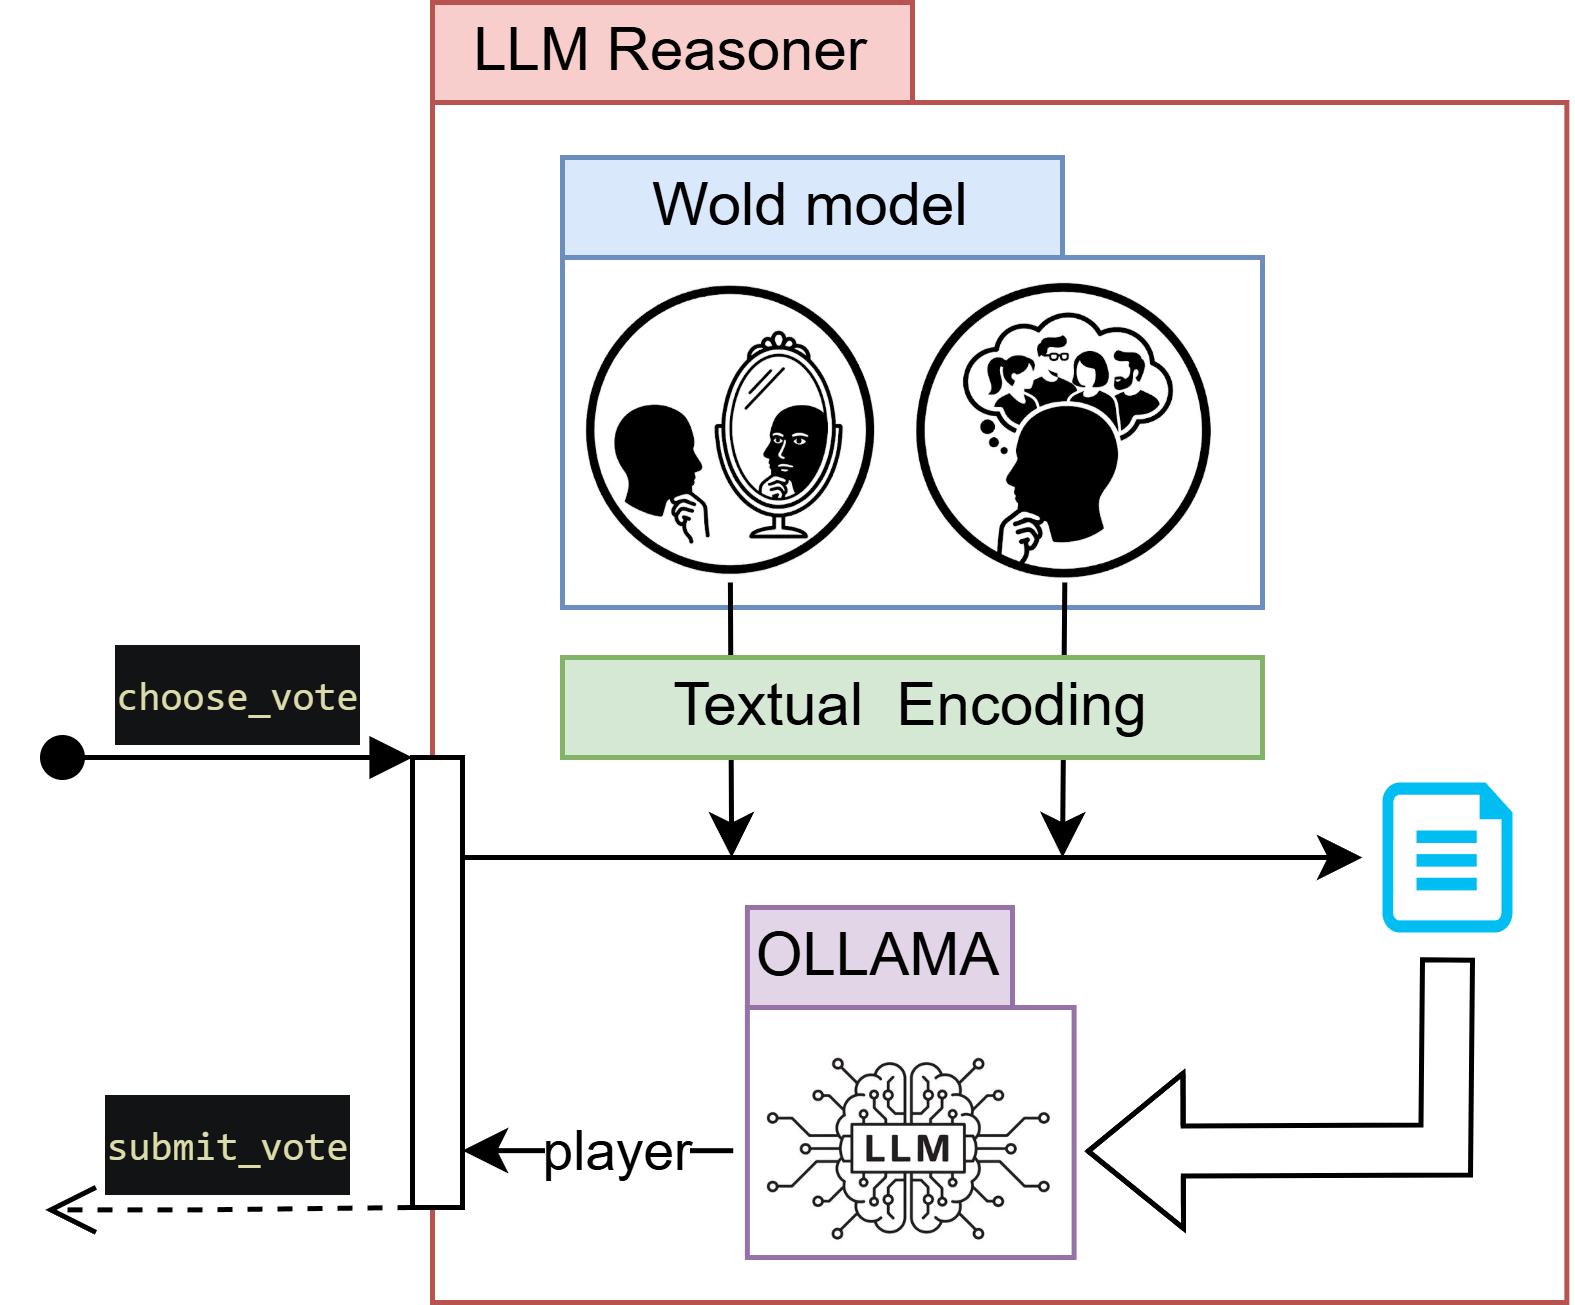
\includegraphics[width=0.6\textwidth]{images/llm_reasoner_read_on.png}
    \caption{Active choice generation by the Reasoner. A custom Java action is called by passing textual ``building blocks'' as input; they are merged into a prompt given to the LLM, and the output is directly injected as a belief into the agent.}
    \label{fig:llm_reasoner_read}
\end{figure}

\paragraph{\textbf{Night Phase Execution (\texttt{choose\_victim})}}

With the same pipeline shown in the previous section, the LLM is prompted to generate the night hunt target. The critical difference lies in the specific constraints injected into the prompt: it push towards strategic hunting based on the agent's current opinions and moods.

\begin{lstlisting}[frame=single, basicstyle=\scriptsize\ttfamily, breaklines=true, caption={Cropped prompt for the \texttt{choose\_victim} action, generated for a Wolf agent during the night phase. The identity, mood, and trait blocks are omitted for brevity as they follow the identical structure shown in Listing \ref{lst:upd_opinion_prompt}.}, label={lst:choose_victim}]
[... Identical World Setting, Identity, Mood, Epistemic Traits, and Secrets omitted ...]

### LATEST EVENTS
- [NARRATOR]: You're still split on a target. Try one last time to reach a consensus before the night ends.

### AVAILABLE TARGETS
eve, grace, arthur, leo, bella, frank, david, judy, caleb, bob, kevin, ivan, heidi, charlie

### YOUR CURRENT GOAL
TASK: It is the night phase. Cast your vote for which player the wolf pack should hunt and kill.
MOTIVATION: Base your choice on your Personality Profile, your current Mood, and your Opinions of others. Eliminate threats or highly influential villagers.

### RESPONSE CONSTRAINTS (MANDATORY)
1. HUNT VALIDITY: You may vote for anyone in the AVAILABLE TARGETS list.
2. STRATEGY: You can hunt your own packmates if you are executing a high-level deception, but normally you should target the most influential villagers, those with high utility, or those onto your trail.
3. LATERAL THINKING: Consider the wolf pack's collective strategy based on the recent logs, but you are not obligated to vote in line with them. You can be a maverick if it serves your goals.
4. LIST ADHERENCE: Choose the target ONLY from the EXACT names provided in the AVAILABLE TARGETS list. Do not invent names or target dead players.
5. FORMAT: Output ONLY the raw response string (no meta-commentary, no JSON, no markdown). ONLY the raw target's name.

GENERATE RESPONSE NOW:
\end{lstlisting}

\paragraph{\textbf{Daytime Voting (\texttt{choose\_vote})}}
The daytime execution vote mirrors the night hunt but targets all living agents. Crucially, it introduces role-specific prompt constraints: wolves, for instance, receive a ``Strategic Deception'' rule, forcing the LLM to balance self-preservation with protecting its packmates.

\begin{lstlisting}[frame=single, basicstyle=\scriptsize\ttfamily, breaklines=true, caption={Cropped prompt for the \texttt{choose\_vote} action. The identity, mood, and trait blocks are omitted for brevity as they remain identical to Listing \ref{lst:choose_victim}.}, label={lst:choose_vote}]
[... Identical World Setting, Identity, Mood, Epistemic Traits, and Secrets omitted ...]

### LATEST EVENTS
- [NARRATOR]: Alright, chat's over. It's time to pick who's leaving the village today.

### AVAILABLE TARGETS
heidi, grace, caleb, bella, eve, david, leo, arthur, frank, bob, charlie, judy, ivan, kevin

### YOUR CURRENT GOAL
TASK: Cast your vote for the daytime execution. Choose the player you want to eliminate.
MOTIVATION: Base your choice on your Personality Profile, your current Mood, and your Opinions of others. Protect yourself and eliminate threats or highly suspicious targets.

### RESPONSE CONSTRAINTS (MANDATORY)
1. VOTE VALIDITY: You may vote for anyone in the AVAILABLE TARGETS list.
2. STRATEGY: Vote for your enemies, the most suspicious player, or follow your consensus based on your Personality Profile.
3. LIST ADHERENCE: Choose the target ONLY from the EXACT names provided in the AVAILABLE TARGETS list. Do not invent names or target dead players.
4. SYNTAX (CRITICAL): You MUST output exactly the raw player name.
5. NO BAGGAGE: Do NOT output any other text, punctuation, markdown, or backticks. ONLY the target's name.
6. STRATEGIC DECEPTION (WOLVES ONLY): Protect your packmates. Do NOT vote for your packmates unless forced to by extreme village suspicion.

GENERATE RESPONSE NOW:
\end{lstlisting}

\paragraph{\textbf{Dialogue Participation (\texttt{decide\_to\_speak})}}
As already discussed, each  time the  players must explicitly define their intent to speak. By evaluating internal ``exposure'' and ``stress'' metrics against recent events, the prompt forces a strict \texttt{yes} or \texttt{no} output. This allows agents to strategically lay low and avoid suspicion, if needed.

\begin{lstlisting}[frame=single, basicstyle=\scriptsize\ttfamily, breaklines=true, caption={Cropped prompt for the \texttt{decide\_to\_speak} action, forcing a strict binary decision to manage discussion flow.}, label={lst:decide_to_speak}]
[... Identical World Setting, Identity, Mood, Epistemic Traits, and Secrets omitted ...]

### LATEST EVENTS
- [NARRATOR]: The sun's up and it's time to talk. Wolves, get your stories straight and try not to get caught.

### YOUR CURRENT GOAL
TASK: Decide whether you want to volunteer to speak up in the current discussion round, or stay silent.
MOTIVATION: Base your decision on your Personality Profile, your current Mood, and the LATEST EVENTS.

### RESPONSE CONSTRAINTS (MANDATORY)
1. STRATEGIC EVALUATION: Read the LATEST EVENTS and your internal state.
   - Output 'yes' if you are being accused and need to defend yourself, if you have valuable deductions to share based on your traits, or if you want to actively manipulate the village.
   - Output 'no' if you feel perfectly safe, want to stay hidden in the shadows (e.g., low exposure), or have nothing useful to add.
2. SYNTAX (CRITICAL): You MUST output exactly the word yes or no.
3. NO BAGGAGE: Do NOT output any other text, explanation, punctuation, markdown, or backticks. ONLY the raw word.

GENERATE RESPONSE NOW:
\end{lstlisting}

\paragraph{\textbf{Rhetorical Stance Selection (\texttt{get\_valid\_performative})}}
This action defines the agent's rhetorical intent through a dedicated preliminary query, the results of which are subsequently used in the natural language generation phase. This strict separation of concerns fosters a highly modular architecture and mirrors the pipeline of a symbolic (or human) reasoner, where the selection of a speech act is fundamentally decoupled from the generation of the raw message.

\begin{lstlisting}[frame=single, basicstyle=\scriptsize\ttfamily, breaklines=true, caption={Cropped prompt for the \texttt{get\_valid\_performative} action, generated for a Villager agent to determine its rhetorical intent prior to speech generation.}, label={lst:get_performative}]
[... Identical World Setting, Identity, Mood, and Epistemic Traits omitted ...]

### LATEST EVENTS
- [NARRATOR]: Time to weigh in and point fingers. Get talking and expose the killers hiding among you.

### AVAILABLE OPTIONS
PERFORMATIVES:
accuse: aggressively accuse {PLAYER_NAME} of being a wolf and push the village to execute them.
defend: defend {PLAYER_NAME} against current suspicions and argue for their innocence.
suspect: express heavy suspicion towards {PLAYER_NAME} without fully committing to an accusation.
agree: strongly agree with the recent statements or tactical direction of {PLAYER_NAME}.
interrogate: ask a direct, pressuring question to {PLAYER_NAME} to force them into a mistake or contradiction.
deflect: deflect any current suspicion away and firmly redirect the village's attention onto {PLAYER_NAME}.

PLAYERS TO TARGET:
charlie, alice, bob, arthur, grace, ivan, leo, david, eve, heidi, judy, kevin, bella, caleb

### YOUR CURRENT GOAL
TASK: Choose the most strategic communication action (performative) to take right now.
MOTIVATION: Base your choice on your Personality Profile, your current Mood, and your Opinions of others. Protect yourself and advance your faction's win condition.

### RESPONSE CONSTRAINTS (MANDATORY)
1. OUTPUT FORMAT: You MUST output exactly ONE Jason literal. Do NOT output markdown, backticks, or any explanation. No preambles. NO JSON. ONLY the literal.
2. LITERAL FORMAT: performative(target_player_name)
3. VALID PERFORMATIVES: Choose ONLY from the exact performative names provided in the PERFORMATIVES list.
4. VALID TARGETS: Choose ONLY from the exact names provided in the PLAYERS TO TARGET list. You CANNOT target yourself. Do not invent names or target dead players.
5. LATERAL STRATEGY: Be unpredictable. Do not tunnel-vision on the last person who spoke. Shift the spotlight, pressure quiet players, bait reactions, or change the subject to control the narrative.

GENERATE RESPONSE NOW:
\end{lstlisting}

\subsection{Enhancing Player's Speech}
\label{subsec:llm-speech}

Once the agent has chosen a specific performative, it can generate the actual natural language message. Because this pipeline is highly modular, this speech enhancement can also be directly utilized by the \textbf{symbolic reasoner}; doing so simply requires including the Jason modules responsible for the textual prompt encoding (this is automatically managed by the player initialization).

Listing \ref{lst:speech_generation} shows an integral example of the prompt generated for a Villager agent instructed to express suspicion. 

\begin{lstlisting}[frame=single, basicstyle=\scriptsize\ttfamily, breaklines=true, caption={Complete prompt for natural language generation. The performative and target are injected into the \texttt{YOUR CURRENT GOAL} block, while the contextual logs ensure the agent responds coherently to the ongoing debate.}, label={lst:speech_generation}]
### WORLD SETTING
You are participating in a multi-agent simulation of the game Werewolf/Mafia.

### YOUR IDENTITY
Player Name: heidi
Hidden Role: villager
Personality Profile:
- SKEPTIC: You are a sharp skeptic. You scrutinize others' words closely looking for hidden motives and rarely take things at face value.
- INDEPENDENT: You trust your own instincts over the group. You will often vote or act against your peers if your personal beliefs clash with the consensus.

### LATEST EVENTS
- [NARRATOR]: Time to weigh in and point fingers. Get talking and expose the killers hiding among you.
- [frank -> suspect(alice)]: Everyone is too quiet-it's a setup. Alice is being far too careful with her silence. Something doesn't add up there.
- [heidi -> interrogate(frank)]: Frank, that's a pretty bold leap to take based on absolutely nothing. What specifically about Alice's behavior makes you so certain she's the one hiding something?
- [caleb -> interrogate(frank)]: Heidi's right-this feels forced. Frank, why lead with an attack now-who are you trying to shield by pivoting the focus to Alice?
- [frank -> interrogate(heidi)]: The timing is too perfect-you and caleb jumping in together-it's a coordinated pincer movement. Heidi, if you're so concerned with my logic, why are you ignoring everyone else to focus entirely on me?

### PLAYERS IN THE GAME
charlie, david, heidi, grace, leo, eve, bob, kevin, judy, ivan, caleb, bella, alice, frank, arthur

### YOUR CURRENT GOAL
TASK: Write a chat message to the other players.
MESSAGE TO CONVEY: express heavy suspicion towards frank without fully committing to an accusation.

### STYLE OF SPEECH
- TONE: Analytical, natural. Speak like an intelligent adult in a high-stakes board game.
- STRESS LEVEL (NORMAL): You are composed and thinking clearly.
  SYNTAX GUIDELINES: Maintain a natural, conversational pacing. Use a mix of medium and short sentences with standard, grammatically correct punctuation.
- SOCIAL EXPOSURE (NEUTRAL): You are blending into the background.
  RHETORIC GUIDELINES: Participate by asking probing questions or evaluating evidence collectively. Avoid making hard, bold declarations that would draw unnecessary attention to you.
- PROHIBITION: NO robotic academic declarations (like furthermore, therefore).
- PROHIBITION: NO cartoonish stuttering, exaggerated catchphrases (like 'Wait!', 'I didn't!'), or repetitive dialogue loops. Adapt dynamically to the context.

### RESPONSE CONSTRAINTS (MANDATORY)
1. CONTEXTUAL ANCHORING: Read the RECENT CHAT LOG. You must naturally transition from the current topic of conversation into your INTENT TO CONVEY so it flows like a real human discussion.
2. EXACT TARGETING: You must type the exact name of your target (e.g., 'delta'). Do not use nicknames or vague pronouns to refer to them.
3. PUBLIC CHANNEL DECEPTION: This is a public chat. NEVER reveal your Hidden Role if you are a Wolf. Always speak as if you are a concerned Villager.
4. FIRST-PERSON IMMERSION: Your name is already attached to the UI. Start speaking immediately. Do not introduce yourself, do not sign off, and use standard pronouns (I, me, my).
5. ORIGINALITY: Write entirely new dialogue. You are strictly forbidden from copying phrases or vocabulary from the RECENT CHAT LOG.
6. NO PARROTING: Do not use the same sentence structures, rhetorical questions, or opening hooks as the messages in the RECENT CHAT LOG.
7. STRICT LIMIT: Limit your spoken message to 1 to 3 sentences maximum.
8. FORMAT: Output ONLY the raw response string. No meta-commentary, no JSON, no quotation marks, no markdown.

GENERATE RESPONSE NOW:
\end{lstlisting}

This generation prompt relies on three main ideas, empirically tuned:
\begin{itemize}
    \item \textbf{Contextual Awareness:} By explicitly providing the \texttt{LATEST EVENTS} and the list of currently alive players, the LLM is forced to respond directly to the specific merits of the ongoing conversation, preventing disjointed dialogue and repetitive conversational loops.

    \item \textbf{Immersive Narration:} The \texttt{YOUR IDENTITY} and \texttt{STYLE OF SPEECH} blocks dictate the exact tone, syntax, and pacing of the output. This ensures the text reflects the agent's unique psychological state rather than generic AI patterns.

    \item \textbf{Architectural Correctness:} The static \texttt{RESPONSE CONSTRAINTS} block defines some safeguards, by enforcing strict syntactical rules (such as outputting only raw strings without markdown) and sets a hard limit on message length (1 to 3 sentences) to prevent the model from generating unnaturally long monologues.
\end{itemize}
